\documentclass[12pt]{article}
\usepackage{tikz}
\usetikzlibrary{arrows.meta, positioning}
\usepackage{amsmath,amssymb}
\usepackage{graphicx}
\usepackage{tcolorbox}
\usepackage{hyperref}
\usepackage{float} 

\begin{document}

\begin{figure}[H]
\centering
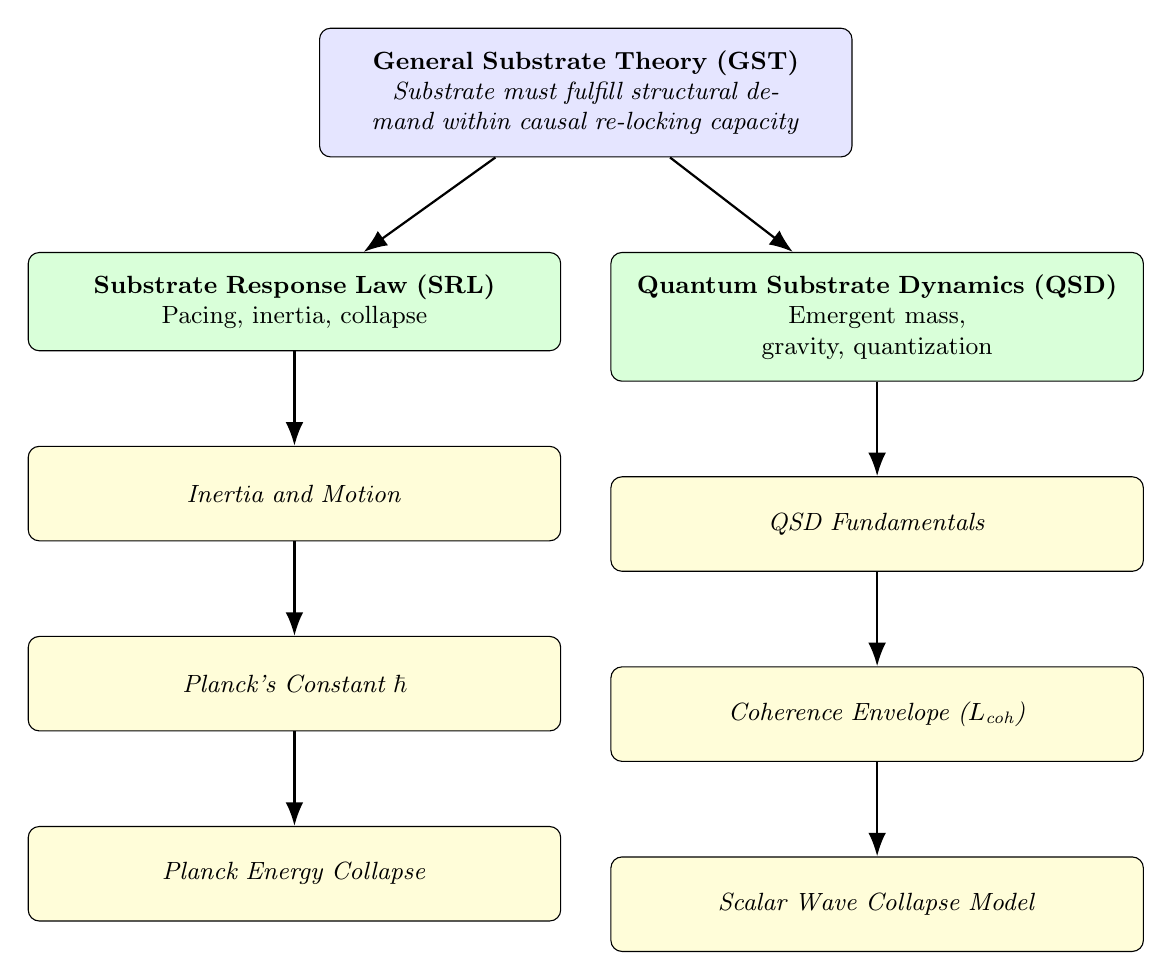
\begin{tikzpicture}[
  box/.style={
    draw, 
    rounded corners, 
    text width=6.2cm, 
    align=center, 
    font=\small,
    minimum height=1.2cm,
    inner sep=8pt
  },
  arr/.style={-{Latex[length=3mm]}, thick},
  node distance=1.2cm
]

% Tier 1 - Root Law
\node[box, fill=blue!10] (gst) {\textbf{General Substrate Theory (GST)}\\ \textit{Substrate must fulfill structural demand within causal re-locking capacity}};

% Tier 2 - Frameworks
\node[box, fill=green!15, below=of gst, xshift=-3.7cm] (srl) {\textbf{Substrate Response Law (SRL)}\\ Pacing, inertia, collapse};
\node[box, fill=green!15, below=of gst, xshift=3.7cm] (qsd) {\textbf{Quantum Substrate Dynamics (QSD)}\\ Emergent mass, \\gravity, quantization};


% Tier 3 - Papers
%\node[box, fill=yellow!15, below=of srl, yshift=-0.3cm] (motion) { \textit{Inertia and Motion}};
%\node[box, fill=yellow!15, below=of qsd, yshift=-0.3cm] (fundamentals) { \textit{QSD Fundamentals}};
\node[box, fill=yellow!15, below=of srl] (motion) { \textit{Inertia and Motion}};
\node[box, fill=yellow!15, below=of qsd] (fundamentals) { \textit{QSD Fundamentals}};

%\node[box, fill=yellow!15, below=of motion, yshift=-0.4cm] (planck) {\textit{Planck’s Constant \(\hbar\)}};
%\node[box, fill=yellow!15, below=of fundamentals, yshift=-0.4cm] (coherence) {\textit{Coherence Envelope (\(L_{\text{coh}}\))}};
%\node[box, fill=yellow!15, below=of planck, yshift=-0.4cm] (ep) {\textit{Planck Energy Collapse}};
%\node[box, fill=yellow!15, below=of coherence, yshift=-0.4cm] (collapse) {\textit{Scalar Wave Collapse Model}};

\node[box, fill=yellow!15, below=of motion] (planck) {\textit{Planck’s Constant \(\hbar\)}};
\node[box, fill=yellow!15, below=of fundamentals] (coherence) {\textit{Coherence Envelope (\(L_{\text{coh}}\))}};
\node[box, fill=yellow!15, below=of planck] (ep) {\textit{Planck Energy Collapse}};
\node[box, fill=yellow!15, below=of coherence] (collapse) {\textit{Scalar Wave Collapse Model}};


% Arrows
\draw[arr] (gst) -- (srl);
\draw[arr] (gst) -- (qsd);
\draw[arr] (srl) -- (motion);
\draw[arr] (motion) -- (planck);
\draw[arr] (qsd) -- (fundamentals);
\draw[arr] (fundamentals) -- (coherence);
\draw[arr] (planck) -- (ep);
\draw[arr] (coherence) -- (collapse);

\end{tikzpicture}
\caption{Structural descent of the QSD theory stack under General Substrate Theory. Each layer inherits from the one above via causal derivation, not heuristic connection.}
\label{fig:theory_stack}
\end{figure}

\end{document}
